\documentclass[12pt]{article}%
\usepackage{amsfonts}
\usepackage{fancyhdr}
\usepackage{comment}
\usepackage[a4paper, top=2.5cm, bottom=2.5cm, left=2.2cm, right=2.2cm]%
{geometry}
\usepackage{times}
\usepackage{amsmath}
\usepackage{changepage}
\usepackage{amssymb}
\usepackage{graphicx}%
\setcounter{MaxMatrixCols}{30}
%\usepackage{hyperref}


%These tell TeX which packages to use.
\usepackage{array,epsfig}
\usepackage{amsmath}
\usepackage{amsfonts}
\usepackage{amssymb}
\usepackage{amsxtra}
\usepackage{amsthm}
\usepackage{mathrsfs}
\usepackage{color}





\usepackage{listings}
\usepackage{longtable}
\definecolor{codegreen}{rgb}{0,0.6,0}
\definecolor{codegray}{rgb}{0.5,0.5,0.5}
\definecolor{codepurple}{rgb}{0.58,0,0.82}
\definecolor{backcolour}{rgb}{0.96,0.96,0.94}
\lstdefinestyle{mystyle}{
	backgroundcolor=\color{backcolour},
	commentstyle=\color{codegreen},
	keywordstyle=\color{blue},
	numberstyle=\tiny\color{codegray},
	stringstyle=\color{codepurple},
	basicstyle=\footnotesize,
	breakatwhitespace=false,
	breaklines=true,
	captionpos=b,
	keepspaces=true,
	numbers=left,
	numbersep=5pt,
	showspaces=false,
	showstringspaces=false,
	showtabs=false,
	tabsize=2
}
\lstset{style=mystyle}

















%%%%%%%%% hyperref %%%%%%%%%%%%
\usepackage[pdftex,letterpaper=true,pdfpagelabels=true,pagebackref=true,bookmarks]{hyperref} 
% with basic options
% pagebackref=true provides links back from the References to the body text. This can cause trouble for printing.

%%%%%%%% cref cleverref %%%%%%%%%%%

% cref package must be loaded after hyperref !
\usepackage[noabbrev]{cleveref}




%Here I define some theorem styles and shortcut commands for symbols I use often
\theoremstyle{definition}
\newtheorem{defn}{Definition}
\newtheorem{thm}{Theorem}
\newtheorem*{thm*}{Theorem}
\newtheorem{cor}{Corollary}
\newtheorem*{rmk}{Remark}
\newtheorem{lem}{Lemma}
\newtheorem*{joke}{Joke}
\newtheorem{ex}{Example}
\newtheorem*{soln}{Solution}
\newtheorem{prop}{Proposition}




\newtheorem{sol}{Solution}


\newtheorem{theorem}{Theorem}
\newtheorem{acknowledgement}[theorem]{Acknowledgement}
\newtheorem{algorithm}[theorem]{Algorithm}
\newtheorem{axiom}{Axiom}
\newtheorem{case}[theorem]{Case}
\newtheorem{claim}[theorem]{Claim}
\newtheorem{conclusion}[theorem]{Conclusion}
\newtheorem{condition}[theorem]{Condition}
\newtheorem{conjecture}[theorem]{Conjecture}
\newtheorem{corollary}[theorem]{Corollary}
\newtheorem{criterion}[theorem]{Criterion}
\newtheorem{definition}[theorem]{Definition}
\newtheorem{example}[theorem]{Example}
\newtheorem{exercise}[theorem]{Exercise}
\newtheorem{lemma}[theorem]{Lemma}
\newtheorem{notation}[theorem]{Notation}
\newtheorem{problem}[theorem]{Problem}
\newtheorem{proposition}[theorem]{Proposition}
\newtheorem{remark}[theorem]{Remark}
\newtheorem{solution}[theorem]{Solution}
\newtheorem{summary}[theorem]{Summary}
%\newenvironment{proof}[1][Proof]{\textbf{#1.} }{\ \rule{0.5em}{0.5em}}

\newcommand{\Q}{\mathbb{Q}}
\newcommand{\R}{\mathbb{R}}
\newcommand{\C}{\mathbb{C}}
\newcommand{\Z}{\mathbb{Z}}


% operators
\DeclareMathOperator{\rank}{{rank}}
\DeclareMathOperator{\argmin}{{argmin}}
\DeclareMathOperator{\argmax}{{argmax}}
\DeclareMathOperator{\flatt}{{flat}}
\DeclareMathOperator{\sym}{{sym}}
\DeclareMathOperator{\sgn}{sgn}
\DeclareMathOperator{\conv}{conv}
\DeclareMathOperator{\env}{env}
\DeclareMathOperator{\dist}{dist}
\DeclareMathOperator{\epi}{epi}
\DeclareMathOperator{\Id}{Id}
\DeclareMathOperator{\dom}{dom}
\DeclareMathOperator{\cl}{cl}
\DeclareMathOperator{\Normal}{Normal}


% matrices
\newcommand{\bbm}{\begin{bmatrix}}
\newcommand{\ebm}{\end{bmatrix}}
\newcommand{\bem}{\begin{pmatrix}}
\newcommand{\eem}{\end{pmatrix}}

% parentheses
%\newcommand{\l[}{\left[}
%\newcommand{\r]}{\right]}
%\newcommand{\l(}{\left(}
%\newcommand{\r)}{\right)}

% 
\def\<{\langle}
\def\>{\rangle}

\usepackage{cite}



%%%%%%%%%%%% Mathcal{ } %%%%%%%
%%%%%%%%%%%%%%%%%%%%%%%%%%%%%%%
\newcommand{\cA}{{\mathcal A}}
\newcommand{\cB}{{\mathcal B}}
\newcommand{\cC}{{\mathcal C}}
\newcommand{\cD}{{\mathcal D}}
\newcommand{\cE}{{\mathcal E}}
\newcommand{\cF}{{\mathcal F}}
\newcommand{\cG}{{\mathcal G}}
\newcommand{\cDQ}{{\mathcal {DQ}}}
\newcommand{\cH}{{\mathcal H}}
\newcommand{\cI}{{\mathcal I}}
\newcommand{\cJ}{{\mathcal J}}
\newcommand{\cK}{{\mathcal K}}
\newcommand{\cL}{{\mathcal L}}
\newcommand{\cM}{{\mathcal M}}
\newcommand{\cN}{{\mathcal N}}
\newcommand{\cO}{{\mathcal O}}
\newcommand{\cP}{{\mathcal P}}
\newcommand{\cQ}{{\mathcal Q}}
\newcommand{\cR}{{\mathcal R}}
\newcommand{\cS}{{\mathcal S}}
\newcommand{\cT}{{\mathcal T}}
\newcommand{\cDP}{{\mathcal {DP}}}
\newcommand{\cU}{{\mathcal U}}
\newcommand{\cV}{{\mathcal V}}
\newcommand{\cW}{{\mathcal W}}
\newcommand{\cX}{{\mathcal X}}
\newcommand{\cY}{{\mathcal Y}}
\newcommand{\cZ}{{\mathcal Z}}

%%%%%%%%%%%% Mathbb{ } %%%%%%%%
%%%%%%%%%%%%%%%%%%%%%%%%%%%%%%%
\newcommand{\bA}{{\mathbb A}}
\newcommand{\bB}{{\mathbb B}}
\newcommand{\bC}{{\mathbb C}}
\newcommand{\bD}{{\mathbb D}}
\newcommand{\bE}{{\mathbb E}}
\newcommand{\bF}{{\mathbb F}}
\newcommand{\bG}{{\mathbb G}}
\newcommand{\bH}{{\mathbb H}}
\newcommand{\bI}{{\mathbb I}}
\newcommand{\bJ}{{\mathbb J}}
\newcommand{\bK}{{\mathbb K}}
\newcommand{\bL}{{\mathbb L}}
\newcommand{\bM}{{\mathbb M}}
\newcommand{\bN}{{\mathbb N}}
\newcommand{\bO}{{\mathbb O}}
\newcommand{\bP}{{\mathbb P}}
\newcommand{\bQ}{{\mathbb Q}}
\newcommand{\bR}{{\mathbb R}}
\newcommand{\bS}{{\mathbb S}}
\newcommand{\bT}{{\mathbb T}}
\newcommand{\bU}{{\mathbb U}}
\newcommand{\bV}{{\mathbb V}}
\newcommand{\bW}{{\mathbb W}}
\newcommand{\bX}{{\mathbb X}}
\newcommand{\bY}{{\mathbb Y}}
\newcommand{\bZ}{{\mathbb Z}}



\begin{document}
	
	\title{CPSC 532W Homework 5}
	\author{Naomi Graham}
	\date{\today}
	\maketitle
	
	All the code can be found on: \url{https://github.com/n6graham/cpsc532_hw5}.
	


	
	\begin{figure}[h]
	\section{Program 1}
	I printed the terminal output from running the unit tests to give incontrovertible proof that they all passed.
	\newline
		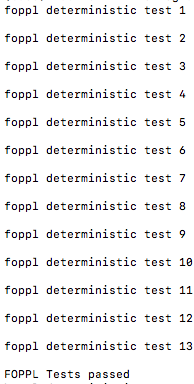
\includegraphics[scale=0.6]{foppl}
		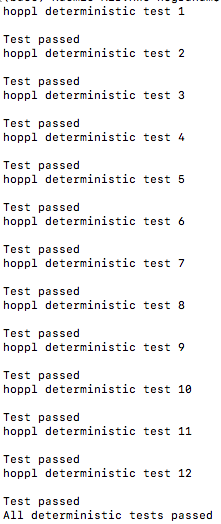
\includegraphics[scale=0.6]{hoppl}
		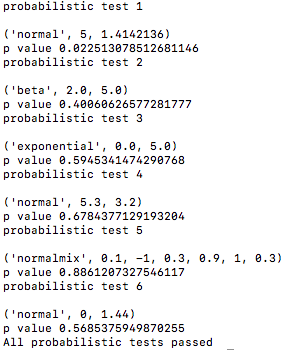
\includegraphics[scale=0.6]{prob}
	\end{figure}
	
	
	\newpage
	
	
	\begin{figure}[h]
	\section{Program 2}
			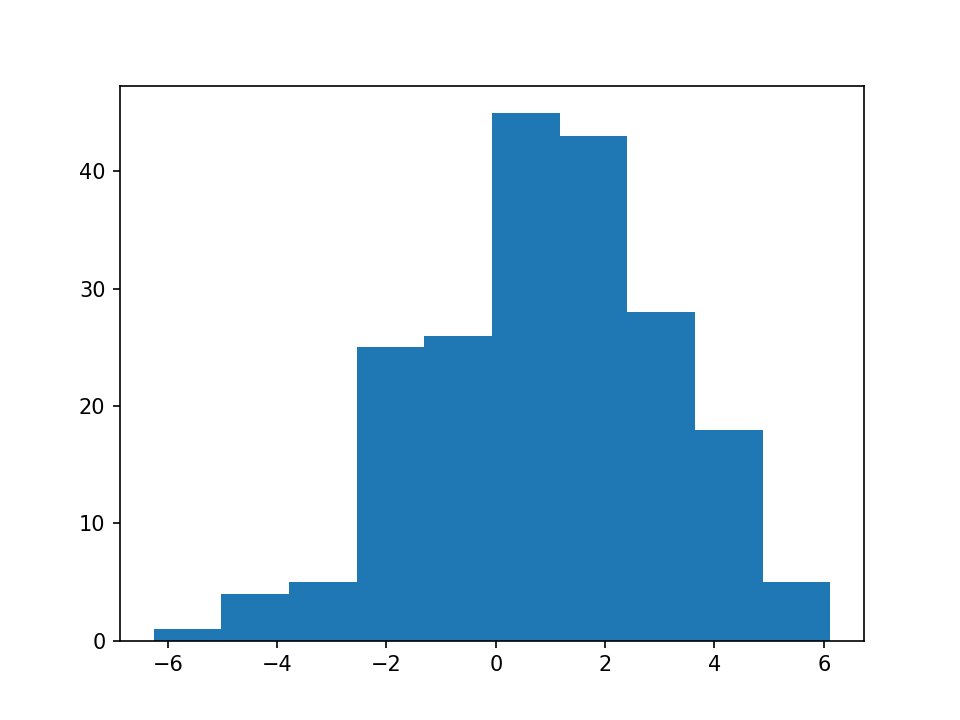
\includegraphics[scale=0.7]{program2_hist}
		\section{Program 3}
		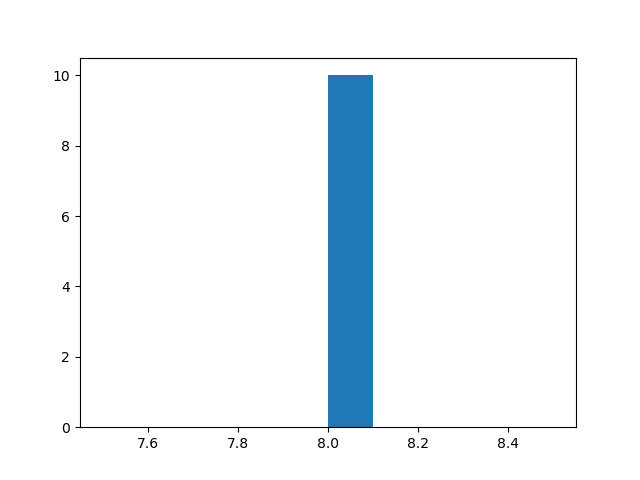
\includegraphics[scale=0.7]{program3_hist}
	\end{figure}
		
	
	

	
	\newpage

	\begin{figure}[h]
	\section{Program 4}
	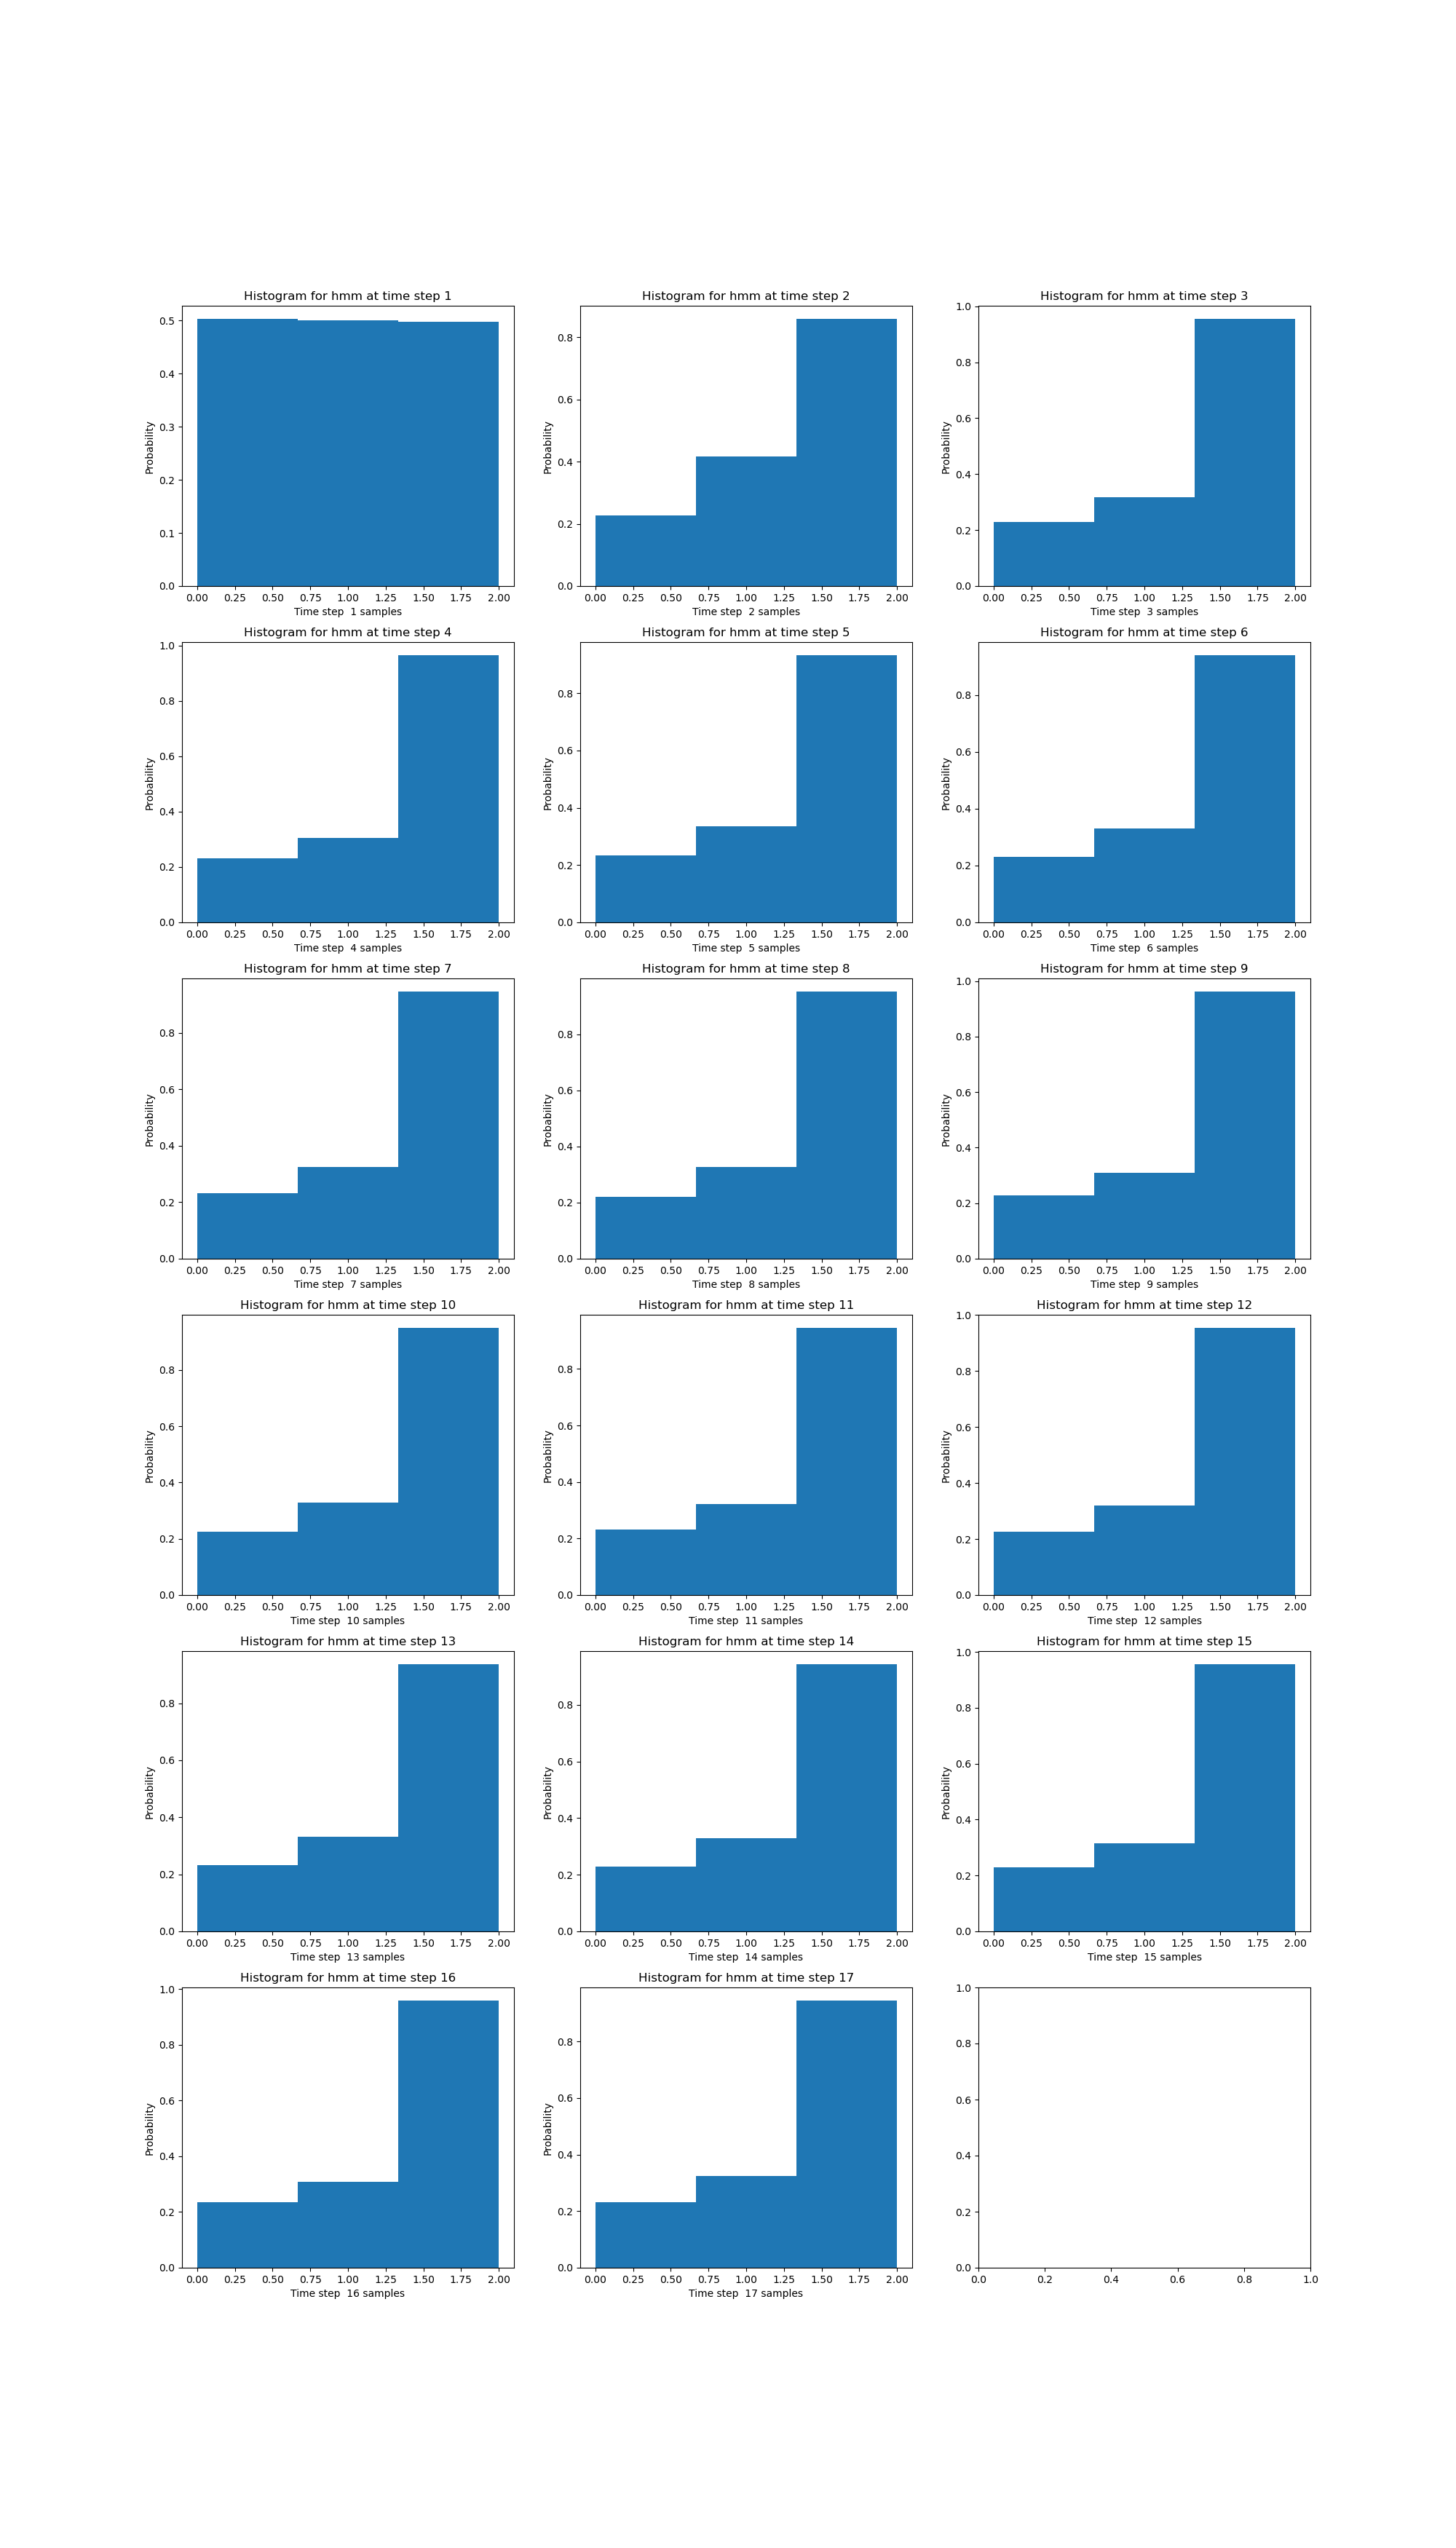
\includegraphics[scale=0.3]{program4_hist}
	\end{figure}
	
	
	\newpage
	
	\section{Snippets of code}
	
	
		\begin{lstlisting}[language=Python]
		class Env(dict):
		    "An environment: a dict of {'var': val} pairs, with an outer Env."
		    def __init__(self, parms=(), args=(), outer=None):
		        self.update(zip(parms, args))
		        self.outer = outer
		        #if outer is not None:
		        #    self.outer = copy.deepcopy(outer)
		    def find(self, var):
		        "Find the innermost Env where var appears."
		        return self if (var in self) else self.outer.find(var)
		    def check_in_env(self, var):
		        return (var in self) or (var in self.outer)
		\end{lstlisting}
		
		
		
		\begin{lstlisting}[language=Python]
		class Lambda(object):
		    "A user-defined Scheme procedure."
		    def __init__(self, parms, body, env):
		        self.parms, self.body, self.env = parms, body, env
		    def __call__(self, *args):
		        return eval(self.body, Env(self.parms, args, self.env)) 
		\end{lstlisting}
			
		
		
		\begin{lstlisting}[language=Python]
		def standard_env() -> Env:
		    env = Env()
		    env.update(pmap(penv))
		    return env
		\end{lstlisting}
		
		
		
		
			
		\begin{lstlisting}[language=Python]
		def eval(expr, envr):
		        
		        if type(expr) is torch.Tensor:
		            return expr
		
		
		        if is_const(expr, envr):
		            if type(expr) in [int, float, bool]:
		                expr = torch.Tensor([expr]).squeeze()
		            elif type(expr) is torch.Tensor:
		                return expr
		            return expr
		
		
		        if type(expr) is str: # and expr != 'fn':    # variable reference
		            try:
		                f = envr.find(expr)[expr]
		                return f
		            except AttributeError:
		                return expr
		
		
		        op, *args = expr
		
		        if is_fn(op,envr):
		            (params, body) = args
		            local_env = Env(outer=envr)
		            lam = Lambda(params,body,local_env)
		            return lam
		
		
		        elif is_if(expr,envr):
		            cond_expr, true_expr, false_expr = args[0], args[1], args[2]
		            tf = eval(cond_expr,envr)
		            res = (true_expr if tf else false_expr)
		            return eval(res,envr)

		
		
		        elif is_sample(expr,envr):
		            dist_expr = args[1]
		            dist_obj = eval(dist_expr,envr)
		            s = dist_obj.sample()
		            return s
		
		
		        elif is_observe(expr,envr):     
		            #dist_expr, obs_expr = args[1], args[2]
		            #dist_obj = eval(dist_expr,envr)
		            #obs_value = eval(obs_expr,envr)
		                            
		            return eval(args[-1],envr)
		
		
		        else:
		            proc=eval(op,envr)
		            vals = [ eval(arg,envr) for arg in args]
		            return proc(*vals)
		\end{lstlisting}
		
		\begin{lstlisting}[language=Python]
		def evaluate(ast, envr=None): 
		    if envr is None:
		        envr = standard_env()
		
		    return eval([ast,'0'],envr) 
		\end{lstlisting}
	
	
	
%	\bibliography{research.bib}
%	\bibliographystyle{plain}
	
	
\end{document}